\documentclass[10pt, leqno]{article}
\usepackage{amsmath}
\usepackage{amsfonts}
\usepackage{amssymb}
%american mathematical society - AMS 
\usepackage{float}
\usepackage{listings}
\lstset{
basicstyle=\small\ttfamily,
columns=flexible,
breaklines=true
}

\usepackage{enumerate}

\usepackage{fullpage}
\usepackage{wrapfig}
\usepackage{subfig}

\oddsidemargin = 0in
\textwidth=6.5in



\usepackage{fullpage}
\usepackage{graphicx}
\usepackage{amsmath}

\providecommand{\e}[1]{\ensuremath{\times 10^{#1}}}

\usepackage{float}

\begin{document}


\begin{centering}

\textbf{Math 448 Homework \#7} \\
Johnny Minor 

\end{centering}
\medskip 

\noindent 3. 

\noindent a. I ran the code for p=1.5 and p=3.0 
\medskip 

\noindent b. We do see quadratic convergence. For the case that p=3.0, for example, we see the norms converge after 7 iterations with the norm of delta u clearly decreasing quadratically. 
\begin{verbatim}
Iteration: 0 and delta u:2.80383508061:
Iteration: 1 and delta u:1.22672147238:
Iteration: 2 and delta u:0.253719993517:
Iteration: 3 and delta u:0.00964730372021:
Iteration: 4 and delta u:1.31690832685e-05:
Iteration: 5 and delta u:2.42260037858e-11:
Iteration: 6 and delta u:1.09498489012e-14:
Iteration: 7 and delta u:6.86034554417e-15:
\end{verbatim}


\noindent c. 
\begin{figure}[H]
  \centering
    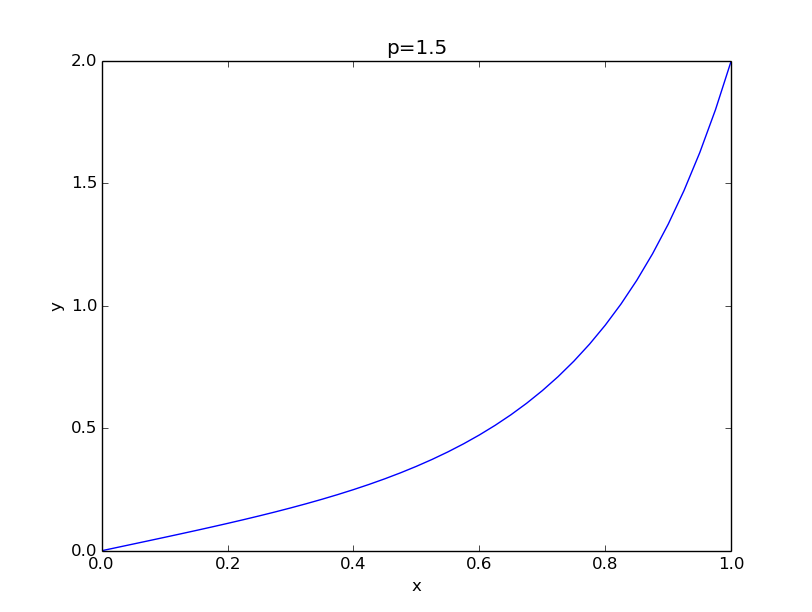
\includegraphics[width=.75\textwidth]{homework7_p15.png}
    \label{fig:s_and_p}
\end{figure}

\begin{figure}[H]
  \centering
    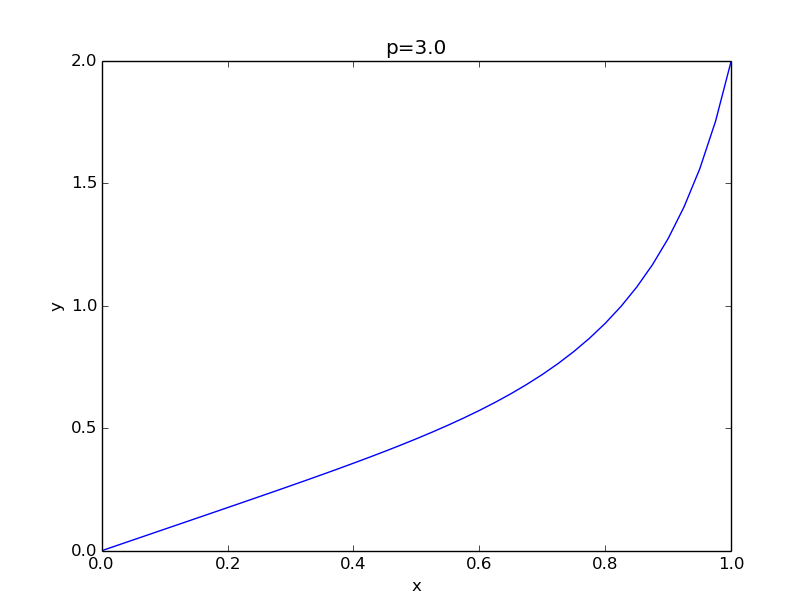
\includegraphics[width=.75\textwidth]{homework7_p30.png}
    \label{fig:s_and_p}
\end{figure}

d. Here's the code I used to generate these: 

\begin{verbatim}
# we are going to solve -u''(x) + 16*u(x)^p = 0
# intial condition of u(0) = 0 and u(1) = 2
# using Newton's method with an initial guess of 2x
# build a mesh on the domain of [0,1]

import numpy as np
import matplotlib.pyplot as plt

left_point = 0.0
right_endpoint = 1.0

p = 3.0  # the power on the u(x) term, the problem is nonlinear when p != 1
n = 40.0  # number of sub intervals
h = 1.0 / n  # sub interval length

x = np.arange(left_point, right_endpoint + h, h)

u = 2.0 * x
print "This is u", u
# when n = 4, then u = [ 0.   0.5  1.   1.5  2. ]

# now we need to create our Jacobian matrix.
# recall that Python is 0 based indexing and MATLAB has 1 based indexing!!!


# Jacobian has -1 on both sides of the main diagonal
diagonals = -1.0*np.ones(n-2)

print diagonals

# storage space
main_diagonal = np.zeros(n-1)

for iteration in np.arange(0, 100):


    for j in np.arange(n-1):
        # print x[i]
        main_diagonal[j] = 2.0 + 16.0 * p * np.power(h, 2.0) * np.power(u[j+1], p - 1.0)
        # print main_diagonal

    jacobian = np.diag(diagonals, -1) + np.diag(diagonals, 1) + np.diag(main_diagonal)

    F = np.zeros(n-1)

    for k in np.arange(1, n):
        F[k-1] = -u[k-1] + 2.0*u[k] - u[k+1] + 16.0 * np.power(h, 2.0) * np.power(u[k], p)


    # now we want to solve the system for delta u
    delta_u = np.linalg.solve(jacobian, -F)

    print "Iteration: {} and delta u:{}:".format(iteration, np.linalg.norm(delta_u))

    for i in np.arange(1, n):
        u[i] += delta_u[i-1]


    if np.linalg.norm(delta_u) < 10e-15:
        print "It took this many iterations", iteration
        break


def hyperbolic_sin(x):
    return 2.0 * np.sinh(4.0*x) / np.sinh(4)


y = hyperbolic_sin(x)
# print "this is y", y
plt.title("p={0}".format(p))
plt.xlabel("x")
plt.ylabel("y")
plt.plot(x, u)
# plt.plot(x, y)
plt.show()

\end{verbatim}


\end{document}